\chapter{Introduction}
\label{cha:Introduction}

Pose and motion estimation of objects is an active field of research due to the growing digitalization of day-to-day processes. A vast majority of existing pose estimation methods take advantage of sensors and markers as indicators for joints. Additionally, the rigid parts of an object and its joints are already known. However, unsupervised methods that are completely independent of user input and detect the pose of an unknown object, constitute a great challenge. Among those methods, the non-rigid registration (see section \ref{nonrigidregistration}) is a well-known approach \cite{survey}.

\begin{figure}[htbp]
	\centering\small
	\begin{tabular}{cc}
		\fbox{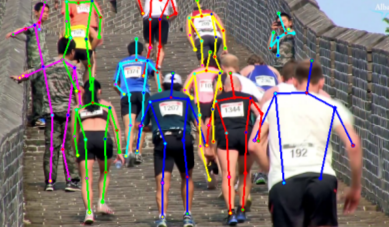
\includegraphics[width=0.43\textwidth]{poseEstimation}} &		% JPEG file
		\fbox{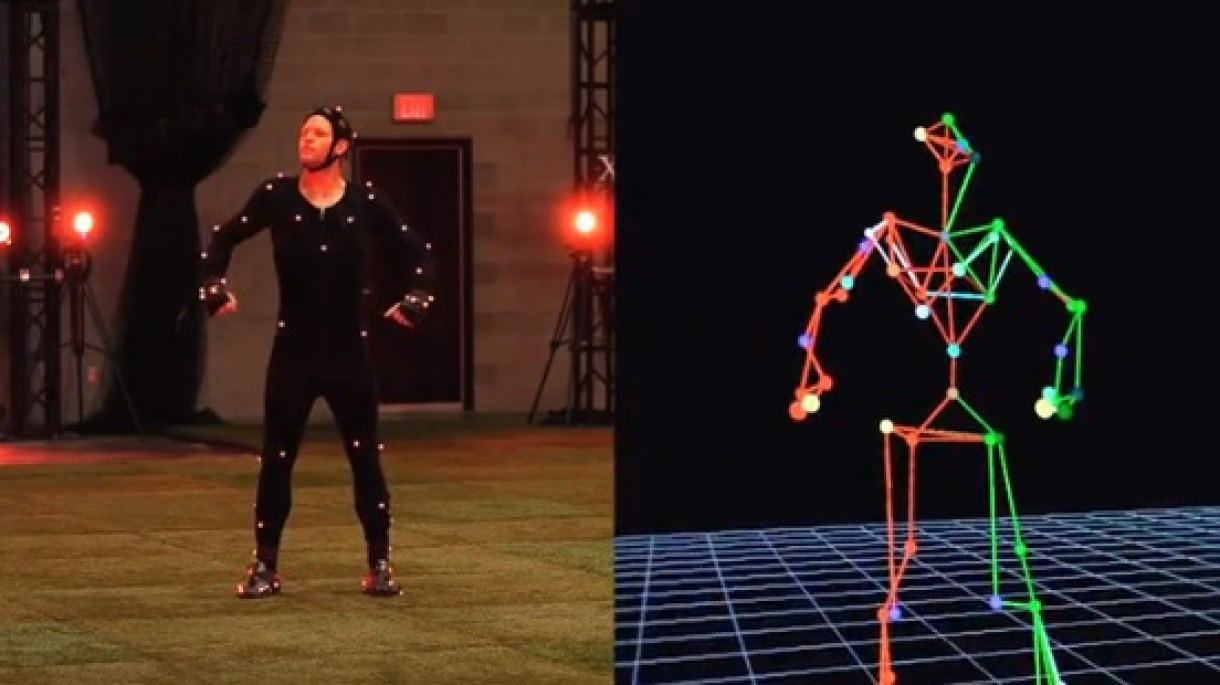
\includegraphics[width=0.45\textwidth]{motionCapture}} 
		\\	% PNG file
		(a) & (b) 
	\end{tabular}
	\caption{Multi-person pose estimation~(a) \cite{poseEstimation} and optical Motion Capture with markers~(b) \cite{MotionCapture}.} 
	\label{fig:motivation}
\end{figure}

\section{Initial idea}

The initial project idea was to create a tool for 3D animation purposes using a small puppet to capture its poses in real-time. However, the idea addressed many different challenges, like 3D reconstruction, segmentation, joint and skeleton estimation as well as creating an interface with a 3D animation program. As the implementation of these tasks would go beyond the scope of a thesis project, it was indispensable to break it down into its main areas. While doing researches on pose estimation, the issue of segmenting an articulated object into its rigid part frequently emerged and for this reason the thesis project focuses on this field. 

\section{General approach}
Generally, there are two major steps to capture the pose of an object. First, bringing the object in 3D, this has to be done to subsequently determine the keypoints (joints). Then the determination of joints and the skeleton takes place. Depending on approach this major step might be subdivided into further steps (shape fitting, segmentation).

IMAGE of steps --> visualized (Real object, 3D visualization, )
How it generally works, examples, not important for this project
examples of 3D scanning

\section{Frequently used approaches of known body parts}
\label{sec:currentApproaches}

How it is done: markers, sensors, shape fitting (already known)
Cite all papers (Voxelization, ....)

\subsection{Markers and sensors}
Many approaches use markers or sensors (Motion Capture) that are placed on the object to be captured. 

ToDo:

- quickly describe methods
- advantages
- disadvantages

\subsection{Shape fitting/Shape from Shilouette}
Rigid parts are known, after Digitalisation of object rigid parts are matched to voxels

\subsection{Other....}
Look over papers!


\section{Unsupervised approaches}

Although the approaches mentioned in section \ref{sec:currentApproaches} work quite well depending on the application, improvements can be made that are more independent from user inputs.... which leads us to the non-rigid registration.

\subsection{Non-rigid registration}
\label{nonrigidregistration}

Generally, registration means the alignment of rigid point clouds (see figure \ref{fig:registration}). A well-known approach to achieve this, is the iterative closest point (ICP) \cite{ICP}, which requires the input point clouds to be aligned quite similar to avoid a local optimum. After registration, a matching error $e$ is achieved, which states the total euclidean distance between the associated points of the registered point clouds. In case of two non-rigid objects (e.g. a human in different poses which is composed of rigid parts) the ICP won't lead to a satisfying registration as associated parts are transformed differently. In order to register a non-rigid object, a segmentation into its rigid parts is required.

\subsection{Challenges}
There are many challenges regarding the non-rigid registration of point clouds in 2D, as well as in 3D. First off, the input data can be noisy by means of points not belonging to the object. Furthermore, the approach is computationally expensive and time-consuming, as the corresponding body parts of two meshes need to be detected iteratively. Additionally, the inevitable difficulty of finding the global optimum, related to ambiguous body parts, has to be overcome.

\begin{figure}[H]
	\centering\small
	\begin{tabular}{cc}
		\fbox{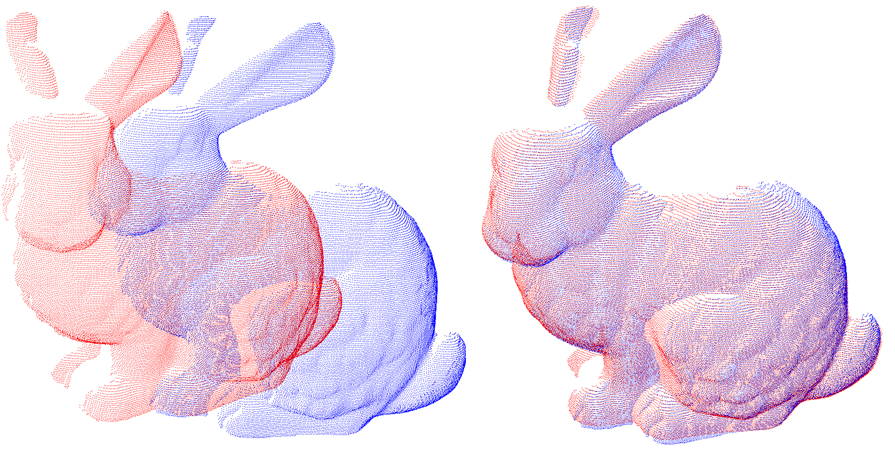
\includegraphics[width=0.43\textwidth]{stanfordBunny}} &		% JPEG file
		\fbox{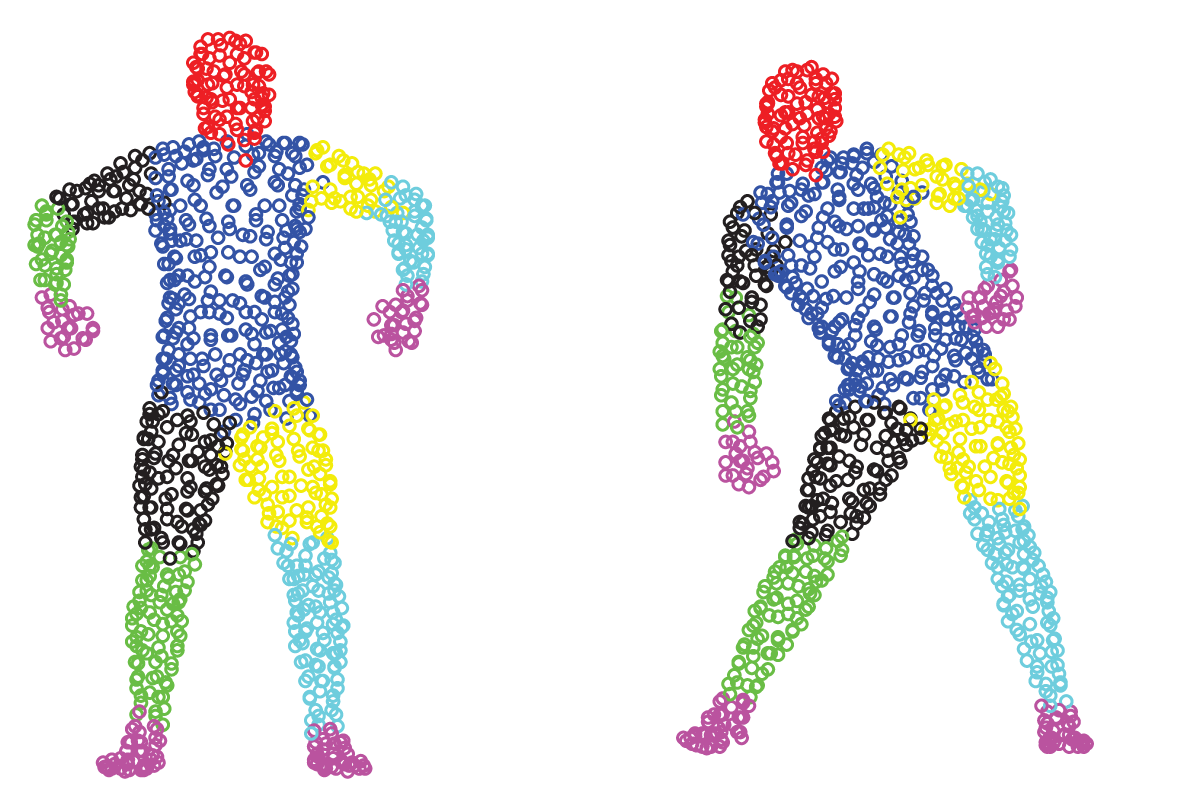
\includegraphics[width=0.45\textwidth]{nonrigidregistration}} 
		\\	% PNG file
		(a) & (b) 
	\end{tabular}
	\caption{Rigid registration of the stanford bunny~(a) \cite{stanfordBunny} and non-rigid registration of a human~(b) \cite{registrationHuman} by detecting its rigid parts.}
	
	\label{fig:registration}
\end{figure}\textbf{}
